\chapter{Especificação de requisitos do trabalho}

\label{CAP4}


% definir técnicas, processos e sistemas, procedimentos que vão compor o sistema

Neste capítulo serão descritas as necessidades básicas levantadas para que o projeto funcione como esperado.

Na figura \ref{fig:class_diagram} pode ser visto o diagrama de classes que define o sistema como um todo.

\begin{figure}[hp]
    \centering
    
    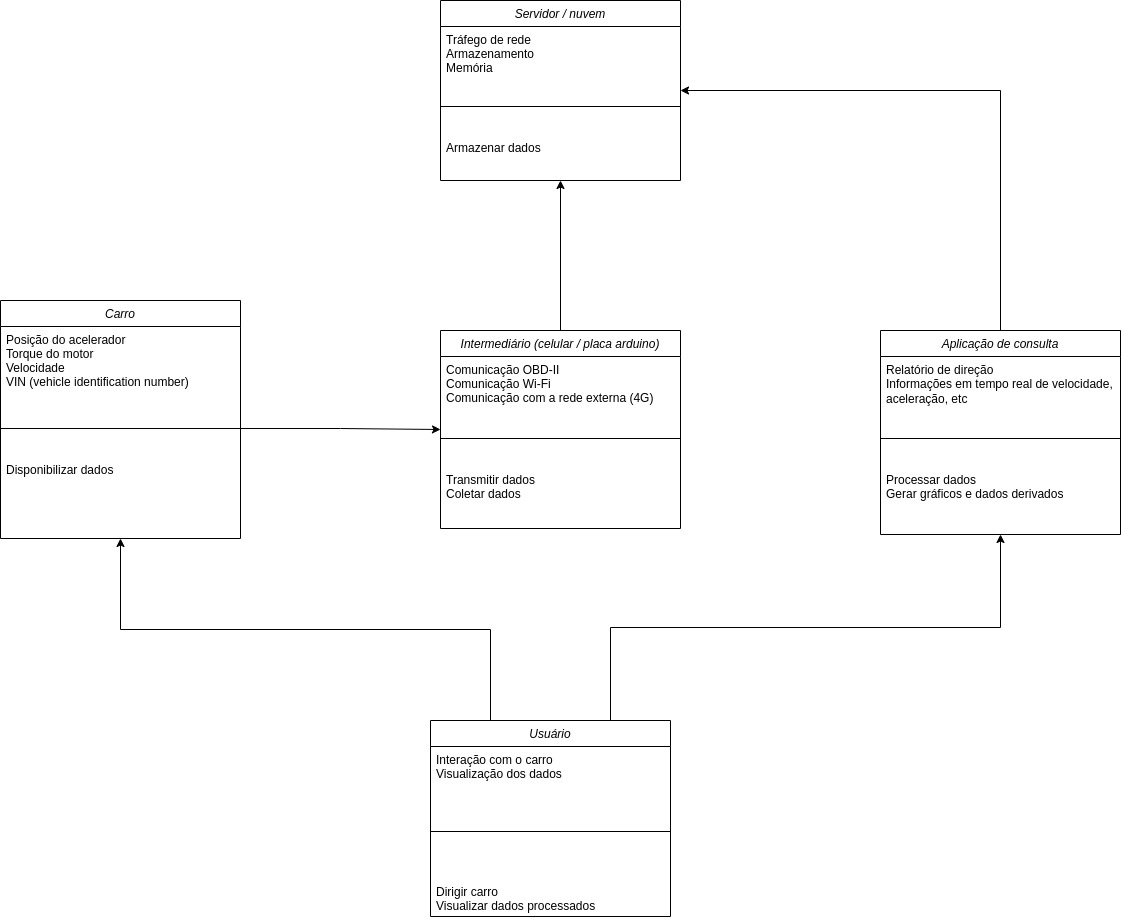
\includegraphics[scale=0.4]{figures/coleta_dados_carro}
    
    \caption{Diagrama de classes com visão mais abstrata do sistema}
    
    \label{fig:class_diagram}
\end{figure}

\section{Requisitos funcionais}
\begin{itemize}
    \item \textbf{Comunicação OBD-II:} fará comunicação com a interface do carro, requisitando apenas as informações definidas, durante o projeto, como relevantes.
    
    \item \textbf{Interface com celular ou módulo de \textit{WiFi}:} deverá estabelecer conexão sem fio com a internet, usando a tecnologia 4G, além de aproveitar-se dos dados de GPS e de aceleração fornecidos pelo celular.
    
    \item \textbf{Plataforma de recepção na nuvem:} utilizando um serviço de armazenamento ainda a ser definido, os dados brutos coletados do carro, do celular (GPS e acelerômetro) e da internet (\textit{Waze}, por exemplo, para informações de tráfego em cada via), assim como as informações depois já processadas, serão todos armazenados na plataforma de \textit{cloud} escolhida.
    
    \item \textbf{\textit{Dashboard} básico informativo:} haverá uma plataforma \textit{Web} que disponibilizará algumas informações básicas para o usuário; deverá ser uma mistura dos dados crus provindos diretamente do carro e também os processados posteriormente, para geração de novas informações também relevantes.
\end{itemize}

\section{Requisitos não-funcionais}

\begin{itemize}
    \item \textbf{Conexão contínua com a internet:} caso a conexão pare por muito tempo, a análise dos dados coletados pode ser prejudicada, além de gerar desconfiança por parte do usuário não havendo garantia de que o sistema é consistente.
    
    \item \textbf{Interface sem reconexão manual com a internet:} se o sistema desligar, a conexão com o celular e com a internet devem ser estabelecidas sem interferência do usuário assim que for ligado novamente; em outras palavras, o sistema deve ser o mais \textit{plug and play} possível.
    
    \item \textbf{Informações relevantes e corretas:} os dados apresentados no \textit{dashboard} precisam ter sentido para o usuário; informações palpáveis como velocidade, aceleração e trajeto percorrido são as únicas que devem chegar até o usuário final, e também precisam passar por algum tipo de "filtro de plausibilidade", para, mais uma vez, não se perder a confiança de quem usará o sistema, apresentando valores \textit{outliers} coletados. 
    
    \item \textbf{Memória e armazenamento em nuvem suficientes:} seja oferecendo espaço ilimitado para o usuário ou definindo um tamanho máximo que pode ser usado, deve ficar claro para o usuário quando e se os seus dados serão apagados do sistema; uma possibilidade seria apagar as informações mais velhas sempre que falte armazenamento.
    
    \item \textbf{Segurança de dados:} pessoas não-autorizadas não pode ter acesso aos dados coletados no veículo de cada usuário.
\end{itemize}

% \subsection{}
% \subsection{}
% \subsection{}


